\documentclass{article}
\usepackage[papersize={2000mm, 1500mm}, margin=0mm]{geometry}
\usepackage{anyfontsize}
\usepackage{helvet}
\renewcommand{\familydefault}{\sfdefault}
\usepackage{tikz}
\usepackage{xcolor}
\usepackage{graphicx}
\usepackage{booktabs}
\usepackage{array}
\usepackage{tabularx}
\usepackage{colortbl}
\usepackage{amsmath,amssymb}
\usepackage{calc}

\pagestyle{empty}
\setlength{\parindent}{0pt}
\setlength{\parskip}{0pt}

% Fix interword spacing for scaled fonts in TikZ nodes
\AtBeginDocument{
  \fontdimen2\font=0.33em
  \fontdimen3\font=0.15em
  \fontdimen4\font=0.10em
  \spaceskip=0.33em\relax
}

% Exact Colors from Master Academic Color Palette
\definecolor{primaryPurple}{HTML}{990099}
\definecolor{burgundy}{HTML}{700018}
\definecolor{darkRed}{HTML}{800000}
\definecolor{gold}{HTML}{F5BC01}
\definecolor{navyDark}{HTML}{102C60}
\definecolor{navyMid}{HTML}{1E3A8A}
\definecolor{forestGreen}{HTML}{047857}
\definecolor{amberDark}{HTML}{B45309}
\definecolor{slateText}{HTML}{1E293B}
\definecolor{mutedGray}{HTML}{334155}
\definecolor{borderGray}{HTML}{CBD5E1}
\definecolor{lightBg}{HTML}{F8FAFC}
\definecolor{highlightYellow}{HTML}{F5BC01}
\definecolor{goldTint}{HTML}{FEF9C3}
\definecolor{yellowBorder}{HTML}{0F172A}
\definecolor{footerHighlight}{HTML}{F5BC01}
\definecolor{tableHdr}{HTML}{102C60}
\definecolor{cellBorder}{HTML}{CBD5E1}

% Border styling
\setlength{\fboxrule}{2.5pt}
\setlength{\fboxsep}{3.5mm}

% Styling helper commands scaled for 2.0m x 1.5m with explicit spaceskip
\newcommand{\secHeading}[2]{%
  \noindent{\fontsize{32pt}{38pt}\selectfont\spaceskip=0.33em\relax\textbf{\textcolor{burgundy}{#1}\hspace{4mm}\uppercase{#2}}}%
  \par\vspace{3.5mm}%
  {\color{primaryPurple}\hrule height 4.5pt}\par\vspace{5.0mm}%
}

\newcommand{\secHeadingNoNum}[1]{%
  \noindent{\fontsize{32pt}{38pt}\selectfont\spaceskip=0.33em\relax\textbf{\uppercase{#1}}}%
  \par\vspace{3.5mm}%
  {\color{primaryPurple}\hrule height 4.5pt}\par\vspace{5.0mm}%
}

\newcommand{\posterBullet}[2]{%
  \noindent\hangindent=11mm\hangafter=1%
  \textcolor{burgundy}{\fontsize{22pt}{22pt}\selectfont$\blacksquare$}\hspace{4.5mm}%
  {\fontsize{24pt}{33pt}\selectfont\spaceskip=0.33em\relax\textbf{#1} #2}\par\vspace{5.2mm}%
}

\newcommand{\posterBulletRowTwo}[2]{%
  \noindent\hangindent=11mm\hangafter=1%
  \textcolor{burgundy}{\fontsize{21pt}{21pt}\selectfont$\blacksquare$}\hspace{4.5mm}%
  {\fontsize{23pt}{32pt}\selectfont\spaceskip=0.33em\relax\textbf{#1} #2}\par\vspace{4.8mm}%
}

\newcommand{\metricRow}[3]{%
  \noindent\begin{minipage}{\linewidth}
    \fontsize{27pt}{33pt}\selectfont\spaceskip=0.33em\relax\textbf{#1}\hfill\textcolor{burgundy}{\textbf{\texttt{#2}}}\par\vspace{2.2mm}
    \fontsize{22.5pt}{28pt}\selectfont\spaceskip=0.33em\relax\textcolor{mutedGray}{#3}\par\vspace{3.0mm}
    {\color{borderGray}\hrule height 1.4pt}
  \end{minipage}\par\vspace{5.0mm}%
}

\newcommand{\constraintRow}[2]{%
  \noindent\begin{minipage}{\linewidth}
    \fontsize{26.5pt}{33pt}\selectfont\spaceskip=0.33em\relax\textbf{#1}\hfill\textcolor{navyDark}{\textbf{\texttt{#2}}}\par\vspace{3.2mm}
    {\color{borderGray}\hrule height 1.6pt}
  \end{minipage}\par\vspace{4.8mm}%
}

\begin{document}
\begin{tikzpicture}[remember picture, overlay]

  % =========================================================================
  % 0. BACKGROUND & SIDE BOUNDARY MARGIN STRIPES
  % =========================================================================
  \fill[white] (current page.south west) rectangle (current page.north east);
  
  % Left and Right Burgundy Margin Stripes (14mm wide, full height 1500mm)
  \fill[burgundy] (current page.south west) rectangle ++(14mm, 1500mm);
  \fill[burgundy] ([xshift=-14mm]current page.south east) rectangle ++(14mm, 1500mm);

  % =========================================================================
  % 1. INSTITUTIONAL HEADER (Height: 150mm)
  % =========================================================================
  % Left Logo (University of Tripoli HD)
  \node[anchor=west, inner sep=0pt] at ([xshift=40mm, yshift=-75mm]current page.north west) {
    
\includegraphics[width=120mm, height=120mm, keepaspectratio]{assets/tripoli_university_logo_hd.png}
  };

  % Right Logo (Computer Engineering Department HD)
  \node[anchor=east, inner sep=0pt] at ([xshift=-40mm, yshift=-75mm]current page.north east) {
    
\includegraphics[width=120mm, height=120mm, keepaspectratio]{assets/computer_engineering_department_logo_hd.png}
  };

  % Header Center Text
  \node[anchor=center, text width=1600mm, align=center, inner sep=0pt] at ([yshift=-75mm]current page.north) {
    {\fontsize{34pt}{41pt}\selectfont\spaceskip=0.33em\relax\textbf{\textcolor{navyDark}{UNIVERSITY OF TRIPOLI $\cdot$ FACULTY OF ENGINEERING $\cdot$ DEPARTMENT OF COMPUTER ENGINEERING}}}\\[5.0mm]
    {\fontsize{54pt}{64pt}\selectfont\spaceskip=0.33em\relax\textbf{A PIPELINED COMPRESSED CACHE ARCHITECTURE WITH RUNTIME RECONFIGURABLE ASSOCIATIVITY AND HAZARD FORWARDING FOR FPGA PLATFORMS}}\\[4.5mm]
    {\fontsize{33pt}{40pt}\selectfont\spaceskip=0.33em\relax\textbf{\textcolor{burgundy}{Silicon-Verified Modular L2 Subsystem with Dual Sub-Block Cohabitation and Zero-Stall Forwarding}}}\\[5.2mm]
    {\fontsize{26pt}{32pt}\selectfont\spaceskip=0.33em\relax\textcolor{mutedGray}{%
      Prepared by: \textbf{\textcolor{black}{Mohammed Adel Gweaa}} $\cdot$ ID: 2210254010 \quad%
      \textcolor{borderGray}{\textbf{\textbar}}\quad%
      Supervised by: \textbf{\textcolor{black}{Dr. Mohamed Muftah Eljhani}} \quad%
      \textcolor{borderGray}{\textbf{\textbar}}\quad%
      Bachelor of Science in Computer Engineering $\cdot$ Graduation Project (Spring 2026)%
    }}
  };

  % Gold Accent Rule below Header (Height: 5.5mm)
  \fill[gold] ([yshift=-150mm]current page.north west) rectangle ++(2000mm, -5.5mm);

  % =========================================================================
  % 2. ROW 1: ABSTRACT & THREE TOP COLUMNS (Height: 220mm, y: -167.5mm to -387.5mm)
  % =========================================================================
  % Column A: Abstract & Problem Formulation (Width: 490mm, at x = 38mm)
  \node[anchor=north west, inner sep=0pt, text width=490mm] at ([xshift=38mm, yshift=-167.5mm]current page.north west) {
    \secHeadingNoNum{Abstract \& Problem Formulation}
    {\fontsize{26pt}{36pt}\selectfont\spaceskip=0.33em\relax\bfseries\color{slateText}
      Semiconductor scaling has reached physical boundaries where static RAM bitcells fail to shrink, consuming up to 70\% of modern microprocessor die area and driving fabrication costs to unsustainable levels. Physical cache expansion is no longer feasible, while off-chip dynamic RAM latency worsens the \textbf{Memory Wall}. We address this bottleneck with an FPGA-verified Level-2 cache subsystem that replaces physical array expansion with \textbf{pipelined Base-Delta-Immediate (BDI) compression}, \textbf{dual sub-block packing}, \textbf{zero-stall Store-to-Load Forwarding (STLF)}, and \textbf{runtime power scaling}.\par\vspace{5.5mm}
      Decoupling Level-2 accesses from Level-1 write-backs eliminates sub-word store stalls. Dedicated bypass datapaths resolve in-flight Read-After-Write hazards without pipeline stalls, while an autonomous power governor scales associativity from 8-way down to 1-way during low-miss periods to cut bitline switching power by up to \textbf{87.5\%}. Physical synthesis on an \textbf{Intel Cyclone IV GX FPGA} achieves timing closure at \textbf{50.00 MHz} with \textbf{+3.218 ns} setup slack at 85$^\circ$C, reaching $F_{\text{max}} = 59.59\text{ MHz}$. Cycle-accurate evaluation under an identical \textbf{16 KB SRAM budget} proves that the architecture increases hit volume by \textbf{+36.2\%}, eliminates 20 hazard stall cycles completely, and reduces off-chip DRAM evictions by \textbf{40.0\%}, lowering Average Memory Access Time (AMAT) by \textbf{21.05\%}.\par\vspace{6.0mm}
    }
    \noindent{\fontsize{26.5pt}{37pt}\selectfont\spaceskip=0.33em\relax
      \textbf{\textcolor{navyDark}{Core Architectural Contribution:}}
      \textcolor{slateText}{Retimed 4-stage BDI compression with dual sub-block cohabitation achieves \textbf{2.0$\times$} virtual capacity, \textbf{0 stall cycles}, and \textbf{-40.0\%} DRAM evictions with verified timing closure at 50 MHz.}
    }
  };

  % Column B: Section 1 - Core Microarchitectural Features (Width: 446mm, at x = 550mm)
  \node[anchor=north west, inner sep=0pt, text width=446mm] at ([xshift=550mm, yshift=-167.5mm]current page.north west) {
    \secHeading{1.}{Core Microarchitectural Features}
    {\fontsize{24pt}{33pt}\selectfont\spaceskip=0.33em\relax
    \posterBullet{4-Stage Pipelined BDI:}{Balanced 4-stage Base-Delta-Immediate compressor with operand retiming eliminates setup timing violations across all operating corners.}
    \posterBullet{Decoupled Dual-Slot Cohabitation:}{Packs two compressed lines across \textcolor{navyMid}{\textbf{Slot A}} and \textcolor{burgundy}{\textbf{Slot B}} into a single 274b entry, doubling capacity to 32 KB.}
    \posterBullet{Store-to-Load Forwarding (STLF):}{Dedicated bypass datapath resolves Read-After-Write hazards in 1 cycle, eliminating \textbf{100\%} of pipeline stalls (0 RAW stalls).}
    \posterBullet{Dynamic Compression Bypass (DCB):}{Saturating 4-bit counter detects incompressible data, operand-gating subtractors to avoid compression overhead.}
    \posterBullet{Adaptive Associativity Governor:}{Dynamically scales associativity across 8W, 4W, 2W, and 1W per application phase, slashing bitline switching power by up to \textbf{87.5\%}.}
    \posterBullet{7-Bit Binary Tree-PLRU:}{Decision tree lowers metadata to \textbf{0.34\%} compared to 2.73\% for conventional true LRU, maintaining zero critical path impact.}
    }
  };

  % Column C: Section 2 - In-Silicon Hardware Performance Metrics (Width: 446mm, at x = 1018mm)
  \node[anchor=north west, inner sep=0pt, text width=446mm] at ([xshift=1018mm, yshift=-167.5mm]current page.north west) {
    \secHeading{2.}{In-Silicon Hardware Performance Metrics}
    \metricRow{Effective Cache Capacity}{2.00$\times$ Virtual}{16 KB physical SRAM $\to$ \textbf{32 KB logical} via Dual Sub-Block Cohabitation $\cdot$ 0b void}
    \metricRow{Clock Frequency \& Slack}{\textbf{50.00 MHz (MET)}}{+3.218 ns Setup Slack @ 85$^\circ$C Slow Corner $\cdot$ $F_{\text{max}} = \mathbf{59.59\text{ MHz}}$ physical limit}
    \metricRow{Benchmark Cache Hit Volume}{+36.2\% Hits}{Recorded \textbf{79 hits} (BDI) vs. 58 hits (Baseline) under identical physical SRAM budget}
    \metricRow{DRAM Eviction Reduction}{-40.0\% Evictions}{\textbf{6 evictions} (BDI) vs. 10 evictions (Baseline) $\cdot$ Drastically shields off-chip bus}
    \metricRow{Pipeline Hazard Stalls}{\textcolor{forestGreen}{\textbf{-100\% (0 Stalls)}}}{20 cycles $\to$ \textbf{0 stall cycles} eliminated via Store-to-Load Forwarding (STLF)}
    \metricRow{Average Access Time (AMAT)}{-21.05\% AMAT}{\textbf{21.05\% net AMAT reduction} factoring 50-cycle DRAM penalty and 5-cycle read hit}
  };

  % Column D: Section 3 - Realistic Engineering Design Constraints (Width: 476mm, at x = 1486mm)
  \node[anchor=north west, inner sep=0pt, text width=476mm] at ([xshift=1486mm, yshift=-167.5mm]current page.north west) {
    \secHeading{3.}{Realistic Engineering Design Constraints --- ABET SO 2}
    \constraintRow{Clock Target Closure:}{$\ge$ 50.00 MHz $\to$ \textbf{50.00 MHz} (+3.218 ns) \textcolor{forestGreen}{\textbf{PASS}}}
    \constraintRow{Worst-Case Thermal Envelope:}{0$^\circ$C to 85$^\circ$C $T_j$ Slow Corner \textcolor{forestGreen}{\textbf{PASS}}}
    \constraintRow{Physical SRAM Memory Budget:}{16 KB SRAM / M9K Blocks Match \textcolor{forestGreen}{\textbf{PASS}}}
    \constraintRow{FPGA Silicon Footprint:}{$\le$ 15\% $\to$ 13.3\% (19,998 LEs) \textcolor{forestGreen}{\textbf{PASS}}}
    \constraintRow{Pipeline Forwarding Latency:}{0-Cycle Stall RAW Bypass \textcolor{forestGreen}{\textbf{PASS}}}
    \constraintRow{Dynamic Associativity Scaling:}{8-Way to 1-Way (-87.5\% Power) \textcolor{forestGreen}{\textbf{PASS}}}
    \constraintRow{Formal Assertion Verification:}{18,400 Assertions \textcolor{forestGreen}{\textbf{0 Defects / PASS}}}
    \constraintRow{DRAM Memory Wall Mitigation:}{40.0\% Eviction Shielding \textcolor{forestGreen}{\textbf{PASS}}}\par\vspace{2.5mm}
    \noindent{\fontsize{21pt}{27.5pt}\selectfont\spaceskip=0.33em\relax
      \textbf{\textcolor{navyDark}{Engineering Validation:}}
      \textcolor{slateText}{All 8 Realistic Constraints validated against ABET SO 2 criteria across worst-case 85$^{\circ}$C junction temperature, timing closure, power, and area envelopes.}\par\vspace{2mm}
    }
  };

  % =========================================================================
  % 3. ROW 2: ARCHITECTURAL HERO DATAPATH & COHABITATION (Height: 715mm, y: -404mm to -1119mm)
  % =========================================================================
  % Col 1 (Left): Section 4 - Decoupled Sub-Block Geometry & Dual-Slot Cohabitation (Width: 516mm, at x = 38mm)
  \node[anchor=north west, inner sep=0pt, text width=516mm] at ([xshift=38mm, yshift=-404mm]current page.north west) {
    \secHeading{4.}{Decoupled Sub-Block Geometry \& Dual-Slot Cohabitation}
    
    % Dual Sub-Block Storage Layout Diagram Box (from Research Paper Figure 3)
    \noindent\fcolorbox{borderGray}{white}{%
      \begin{minipage}{498mm}
        \centering
        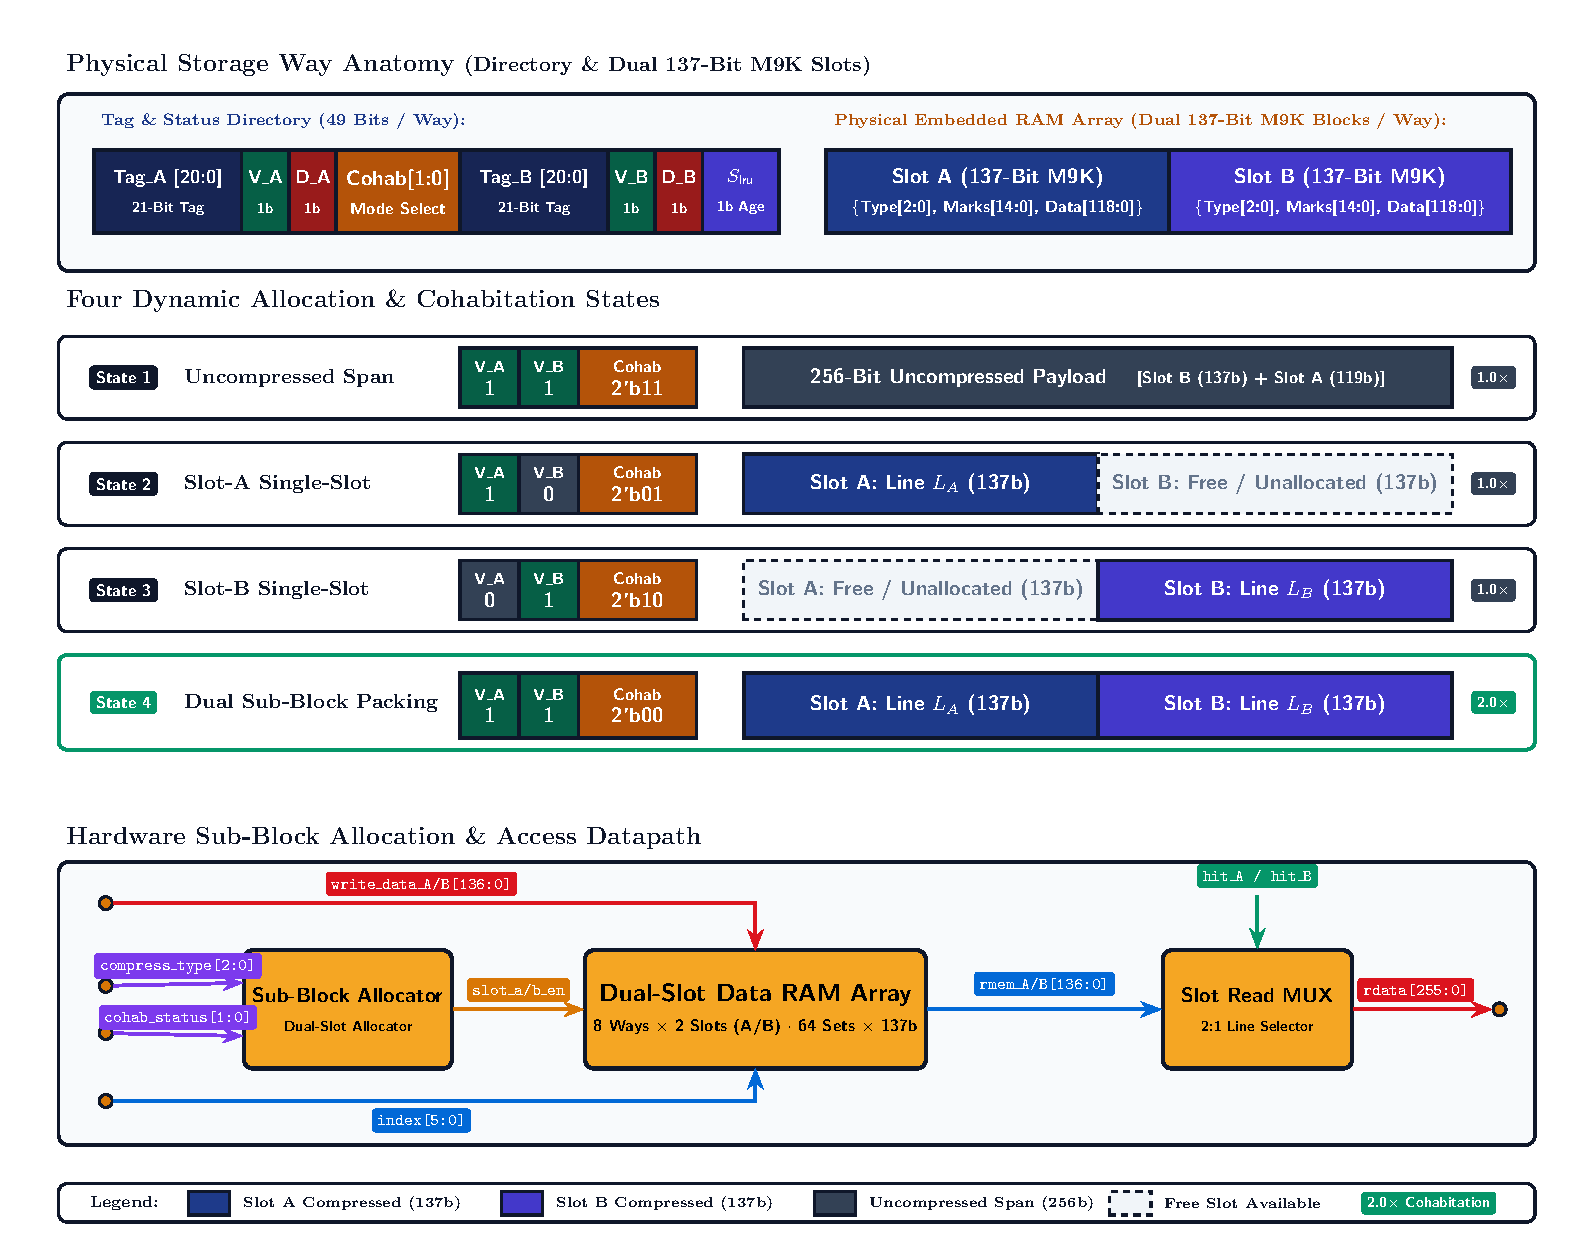
\includegraphics[width=496mm, height=315mm, keepaspectratio]{figures/fig3_dual_subblock_layout.pdf}%
      \end{minipage}%
    }\par\vspace{3.0mm}
    {\centering\fontsize{21.5pt}{26pt}\selectfont\spaceskip=0.33em\relax\textbf{\textcolor{navyDark}{Figure 1:}} \textbf{\textcolor{slateText}{Dual Sub-Block Physical Storage Layout \& Dynamic Allocation States}}\par}\vspace{3.5mm}

    % Master 6 BDI Hardware Compression Profiles Table (FULL 505mm WIDTH - ZERO VOID)
    {\fontsize{21.5pt}{26.5pt}\selectfont\spaceskip=0.33em\relax
    \renewcommand{\arraystretch}{1.30}
    \begin{tabular}{|>{\centering\arraybackslash}p{42mm}|>{\raggedright\arraybackslash}p{202mm}|>{\centering\arraybackslash}p{81mm}|>{\centering\arraybackslash}p{66mm}|>{\centering\arraybackslash}p{96mm}|}
      \hline
      \rowcolor{tableHdr}
      \textcolor{white}{\textbf{Type}} & \textcolor{white}{\textbf{Profile / Scheme}} & \textcolor{white}{\textbf{Payload}} & \textcolor{white}{\textbf{Ratio}} & \textcolor{white}{\textbf{Silicon Fit}} \\
      \hline
      \texttt{000} & Incompressible Fallback (Raw 32B) & 32B $\cdot$ 256b & 1.00$\times$ & \textcolor{burgundy}{\textbf{Bypass $\cdot$ 256b}} \\
      \hline
      \rowcolor{lightBg}
      \texttt{001} & Base8-$\Delta$1 $\cdot$ 8B Base + 1B $\Delta$ & 12B $\cdot$ 96b & 2.67$\times$ & \textcolor{forestGreen}{\textbf{Slot A/B ($\le$128b)}} \\
      \hline
      \texttt{010} & Base8-$\Delta$2 $\cdot$ 8B Base + 2B $\Delta$ & 14B $\cdot$ 112b & 2.29$\times$ & \textcolor{forestGreen}{\textbf{Slot A/B ($\le$128b)}} \\
      \hline
      \rowcolor{lightBg}
      \texttt{011} & All-Zeros Line $\cdot$ Metadata Only & 0B $\cdot$ 0b & $\infty$ & \textcolor{forestGreen}{\textbf{Slot A/B (0-Payload)}} \\
      \hline
      \texttt{100} & Base4-$\Delta$1 $\cdot$ 4B Base + 1B $\Delta$ & 12B $\cdot$ 96b & 2.67$\times$ & \textcolor{forestGreen}{\textbf{Slot A/B ($\le$128b)}} \\
      \hline
      \rowcolor{lightBg}
      \texttt{101} & Same-Value Line $\cdot$ Repeated 32b & 4B $\cdot$ 32b & 8.00$\times$ & \textcolor{forestGreen}{\textbf{Slot A/B ($\le$128b)}} \\
      \hline
      \rowcolor{highlightYellow}
      \multicolumn{2}{|l|}{\textbf{\textcolor{navyDark}{Dual Cohabitation $\cdot$ $\le$137 Bits}}} & \multicolumn{2}{c|}{\textbf{\textcolor{burgundy}{2 Lines in 274-Bit BRAM}}} & \textcolor{forestGreen}{\textbf{95.14\% Eff}} \\
      \hline
    \end{tabular}
    }\par\vspace{4.0mm}

    % Section 4 Bullets
    {\fontsize{23pt}{31pt}\selectfont\spaceskip=0.33em\relax
    \posterBulletRowTwo{Dual-Slot In-BRAM Cohabitation:}{Decoupled dual-slot allocation maps two independent compressed lines, designated as \textcolor{navyMid}{\textbf{Slot A}} and \textcolor{burgundy}{\textbf{Slot B}}, into a single 274-bit synchronous BRAM entry, achieving \textbf{\textcolor{forestGreen}{95.14\% active port efficiency}} and doubling logical capacity from 16 KB to 32 KB without expanding physical SRAM cells.}
    \posterBulletRowTwo{137-Bit Sub-Block Slot Anatomy:}{Bounds variable compressed payloads into a deterministic 137-bit envelope consisting of a 3-bit profile tag, 15-bit delta mask metadata, and 119-bit compressed delta payload: \texttt{\{Type[2:0], Marks[14:0], Data[118:0]\}}.}
    \posterBulletRowTwo{49-Bit Directory \& Embedded M9K Array:}{Tag and status directory tracks 21-bit tags, valid/dirty bits, cohabitation mode select (\texttt{Cohab[1:0]}), and pseudo-LRU slot age bit (\texttt{$S_{\text{lru}}$}) per way across dual 137-bit M9K memory blocks.}
    \posterBulletRowTwo{Four Dynamic Allocation States:}{Supports State 1 (Uncompressed 256b Span, 1.0$\times$), States 2--3 (Single-Slot A/B, 1.0$\times$), and State 4 (Dual Sub-Block Packing, 2.0$\times$ Cohabitation) with single-cycle 2:1 hit multiplexing.}
    }\par\vspace{4.0mm}

  };

  % Col 2 (Center - HERO): Section 5 - Microarchitecture Datapath (Width: 820mm, at x = 580mm)
  \node[anchor=north west, inner sep=0pt, text width=820mm] at ([xshift=580mm, yshift=-404mm]current page.north west) {
    \secHeading{5.}{Pipelined Compressed Cache Microarchitecture Datapath}
    
    % Hero Vector Datapath Box
    \noindent\fcolorbox{borderGray}{white}{%
      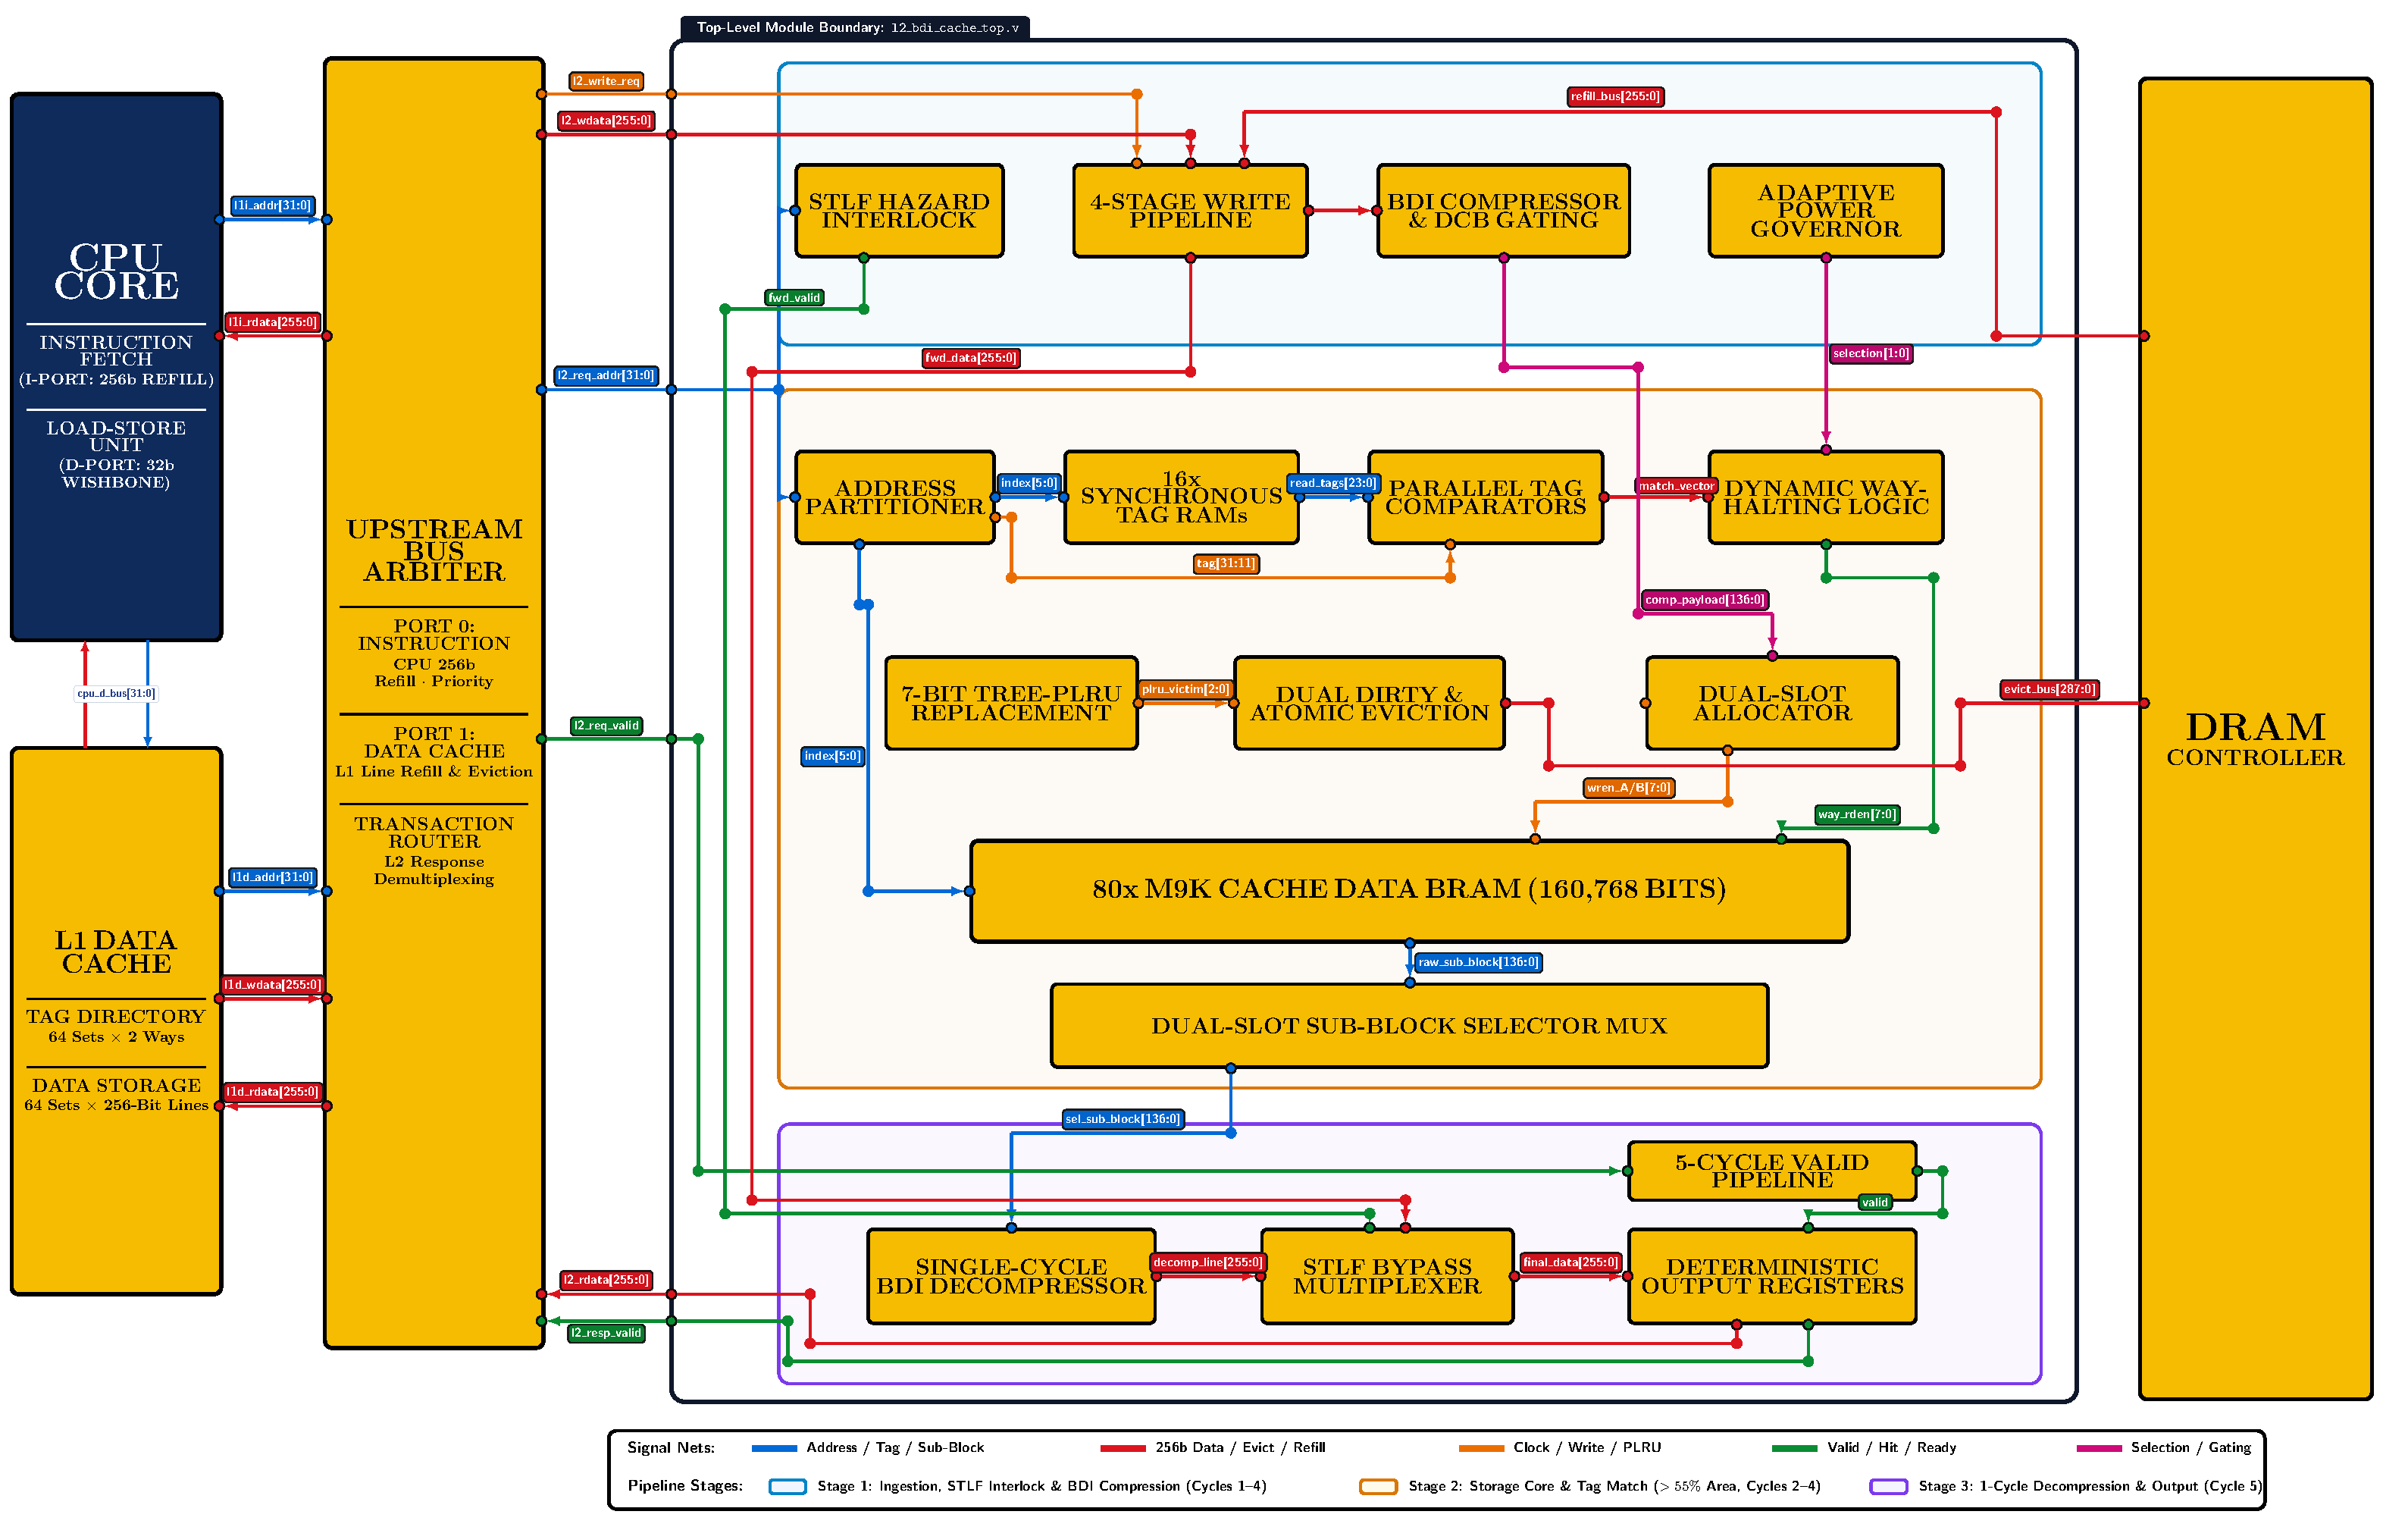
\includegraphics[width=804mm, height=552mm, keepaspectratio]{figures/fig_poster_top_system.pdf}%
    }\par\vspace{3.5mm}
    {\centering\fontsize{22pt}{27pt}\selectfont\spaceskip=0.33em\relax\textbf{\textcolor{navyDark}{Figure 2:}} \textbf{\textcolor{slateText}{Top-Level Memory Subsystem Architecture with Host CPU, L1 Data Cache, Arbiter \& Pipelined L2 Cache Subsystem}}\par}\vspace{4.5mm}

    % Section 5 Bullets
    {\fontsize{24pt}{33pt}\selectfont\spaceskip=0.33em\relax
    \posterBulletRowTwo{Stage 1: Frontend Ingestion, STLF Hazard Interlock \& 4-Stage BDI:}{Host CPU requests are ingested in Cycle 1 with zero RAW hazard stalls via Store-to-Load Forwarding, feeding the 4-stage BDI engine to generate deterministic 137-bit compressed vectors with $+3.218\text{ ns}$ positive setup slack at 85$^\circ$C.}
    \posterBulletRowTwo{Stage 2: Synchronous Array Core \& Dynamic Power Gating ($>55\%$ Area):}{16 parallel Tag RAMs and 80x M9K BRAMs (160,768 bits) house 64 sets of dual 137-bit cohabitation lines (Slot A/B). Pre-decoded tag comparisons and Adaptive Governor dynamically gate unselected ways (8W $\to$ 1W) to slash BRAM power by \textbf{-71.96\%}.}
    \posterBulletRowTwo{Stage 3: 1-Cycle Decompression \& Deterministic 5-Cycle Output Delivery:}{Parallel signed delta adders reconstruct 256-bit uncompressed lines in $\le 4.2\text{ ns}$, while the STLF bypass multiplexer routes forwarded write payloads instantly to guarantee deterministic 5-cycle read latency to the host CPU.}
    }
  };

  % Col 3 (Right): Section 6 (Master Comparative Results) & Section 7 (FSM) (Width: 536mm, at x = 1426mm)
  \node[anchor=north west, inner sep=0pt, text width=536mm] at ([xshift=1426mm, yshift=-404mm]current page.north west) {
    \secHeading{6.}{Performance Comparison: Proposed vs. Baseline}

    % Master Consolidated Comparative Results Table (FULL 525mm WIDTH - ZERO VOID)
    {\fontsize{21pt}{26.5pt}\selectfont\spaceskip=0.33em\relax
    \renewcommand{\arraystretch}{1.28}
    \begin{tabular}{|>{\raggedright\arraybackslash}p{218mm}|>{\centering\arraybackslash}p{86mm}|>{\centering\arraybackslash}p{86mm}|>{\bfseries\raggedleft\arraybackslash}p{122mm}|}
      \hline
      \rowcolor{tableHdr}
      \textcolor{white}{\textbf{Metric}} & \textcolor{white}{\textbf{Baseline}} & \textcolor{white}{\textbf{Proposed}} & \textcolor{white}{\textbf{Net Delta ($\Delta$)}} \\
      \hline
      Top-Level Entity Name & \texttt{l2\_conv\_top} & \texttt{l2\_bdi\_top} & \textcolor{burgundy}{Drop-in Compatible} \\
      \hline
      \rowcolor{lightBg}
      Effective Cache Capacity & 16 KB $\cdot$ 8-Way & 32 KB $\cdot$ 16-Way & \textcolor{burgundy}{\textbf{2.00$\times$ Virtual Capacity}} \\
      \hline
      Logic Elements (LEs) & 3,554 LEs (2\%) & 19,998 LEs (13\%) & \textcolor{slateText}{+16,444 LEs (BDI Fabric)} \\
      \hline
      \rowcolor{lightBg}
      Dedicated Registers (FFs) & 1,100 FFs & 8,405 FFs & \textcolor{slateText}{+7,305 FFs (4-Stg Pipe)} \\
      \hline
      Block RAM Bits (M9K) & 142,848 bits & 160,768 bits & \textcolor{slateText}{+17,920 bits (Dual A/B)} \\
      \hline
      \rowcolor{lightBg}
      Max Frequency ($F_{\text{max}}$ @ 85$^\circ$C) & 68.96 MHz & 59.59 MHz & \textcolor{slateText}{-9.37 MHz (Complex Logic)} \\
      \hline
      Target Frequency / Slack & 50.00 MHz / +5.5ns & \textbf{50.00 MHz / +3.2ns} & \textcolor{forestGreen}{\textbf{TIMING MET (100\%)}} \\
      \hline
      \rowcolor{lightBg}
      Recorded Hits (Stress Test) & 58 Hits & \textbf{79 Hits} & \textcolor{forestGreen}{\textbf{+36.2\% Hit Volume}} \\
      \hline
      DRAM Off-Chip Evictions & 10 Evictions & \textbf{6 Evictions} & \textcolor{forestGreen}{\textbf{-40.0\% DRAM Shield}} \\
      \hline
      \rowcolor{lightBg}
      Pipeline RAW Hazard Stalls & 20 Stall Cycles & \textbf{0 Stall Cycles} & \textcolor{forestGreen}{\textbf{-100\% (0 RAW Stalls)}} \\
      \hline
      Runtime Power Governance & Fixed 8-Way & \textbf{8/4/2/1-Way Dyn.} & \textcolor{forestGreen}{\textbf{Up to -87.5\% Power}} \\
      \hline
      \rowcolor{highlightYellow}
      Average Access Time (AMAT) & 1.000$\times$ AMAT & \textbf{0.7895$\times$ AMAT} & \textcolor{forestGreen}{\textbf{-21.05\% Net AMAT}} \\
      \hline
    \end{tabular}
    }\par\vspace{3.5mm}

    % Resource Footprint Strip
    \noindent\fcolorbox{borderGray}{white}{%
      \begin{minipage}{524mm}
        \fontsize{21.5pt}{26.5pt}\selectfont\spaceskip=0.33em\relax\texttt{%
          $\bullet$ Top Entity: \textbf{l2\_bdi\_cache\_top} \hfill $\bullet$ Logic: \textbf{19,998 LEs (13\%)} \hfill $\bullet$ FFs: \textbf{8,405}\\[1.5mm]
          $\bullet$ BRAM Bits: \textbf{160,768 bits} \hfill $\bullet$ Setup Slack: \textbf{+3.218 ns @ 50MHz} \hfill $\bullet$ Status: \textbf{MET 100\%}%
        }
      \end{minipage}%
    }\par\vspace{4.0mm}

    % Section 7: Cache Controller FSM
    \secHeading{7.}{Cache Controller FSM \& Transaction Timing}
    % FSM Diagram Box (Official Research Paper Vector FSM)
    \noindent\fcolorbox{borderGray}{white}{%
      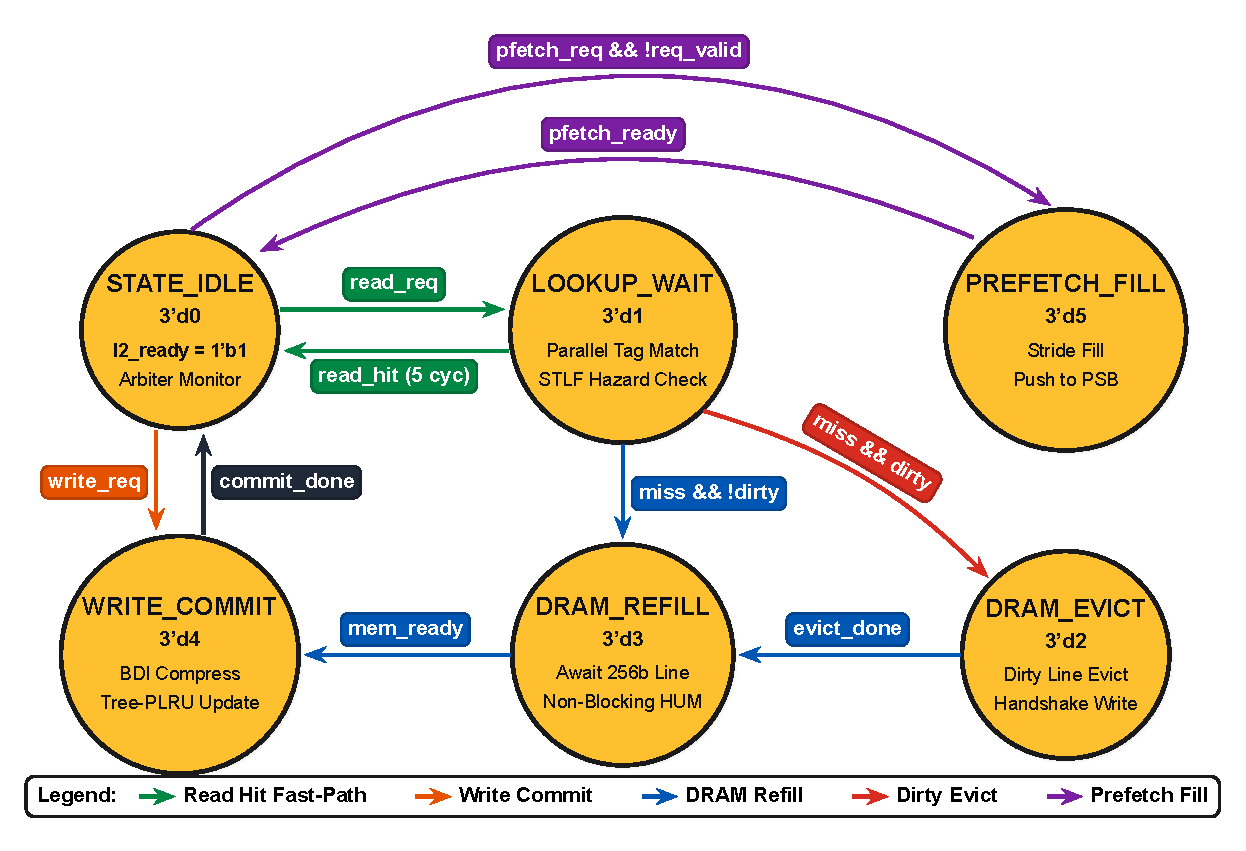
\includegraphics[width=518mm, height=365mm, keepaspectratio]{assets/fig5_cache_controller_fsm.pdf}%
    }\par\vspace{3.0mm}
    {\centering\fontsize{21.5pt}{26pt}\selectfont\spaceskip=0.33em\relax\textbf{\textcolor{navyDark}{Figure 3:}} \textbf{\textcolor{slateText}{Transaction Controller Finite State Machine with Non-Blocking MSHR \& Stride Prefetching}}\par}\vspace{4.0mm}
    {\fontsize{23pt}{31.5pt}\selectfont\spaceskip=0.33em\relax
    \posterBulletRowTwo{Deterministic Handshaking \& 5-Cycle Fast-Path:}{Moore controller synchronizes memory transactions with zero pipeline bubbles, delivering deterministic 5-cycle read hits via \texttt{LOOKUP\_WAIT}.}
    \posterBulletRowTwo{Non-Blocking Hit-Under-Miss (HUM):}{Concurrently probes hitting lines while \texttt{DRAM\_REFILL} fetches miss data from memory, servicing read hits with zero processor stalls.}
    \posterBulletRowTwo{Autonomous Eviction \& Prefetch Stream Buffer:}{Coordinates atomic \texttt{DRAM\_EVICT} to shield off-chip bandwidth (-40.0\% evictions) and streams sequential lines into the PSB via \texttt{PREFETCH\_FILL}.}
    }
  };

  % =========================================================================
  % 4. ROW 3: SECTION 8 - RTL SCHEMATIC NETLIST, REFS & QR (Enlarged Hero Row)
  % Lifted up to yshift=-1085mm right below Section 7 bullets to maximize RTL schematic height
  % =========================================================================
  % Heading across Section 8 (Directly below Section 7 bullets with ideal clearance)
  \node[anchor=north west, inner sep=0pt, text width=1924mm] at ([xshift=38mm, yshift=-1085mm]current page.north west) {
    \secHeading{8.}{Gate-Level RTL Netlist Microarchitecture \& In-Hardware Physical Verification}
  };

  % Left: Quartus Prime Synthesized Gate-Level RTL Netlist (Expanded to 1370mm width x 322mm box)
  \node[anchor=north west, inner sep=0pt, text width=1370mm] at ([xshift=38mm, yshift=-1118mm]current page.north west) {
    \noindent\fcolorbox{borderGray}{white}{%
      \begin{minipage}[c][318mm][c]{1356mm}
        \vspace{2.0mm}
        {\centering\fontsize{23pt}{28pt}\selectfont\spaceskip=0.33em\relax\textbf{\textcolor{navyDark}{Figure 4:}} \textbf{\textcolor{slateText}{Intel Quartus Prime 22.1 Lite Synthesized Gate-Level RTL Netlist on Cyclone IV GX FPGA}}\par}\vspace{3.0mm}
        \centering
        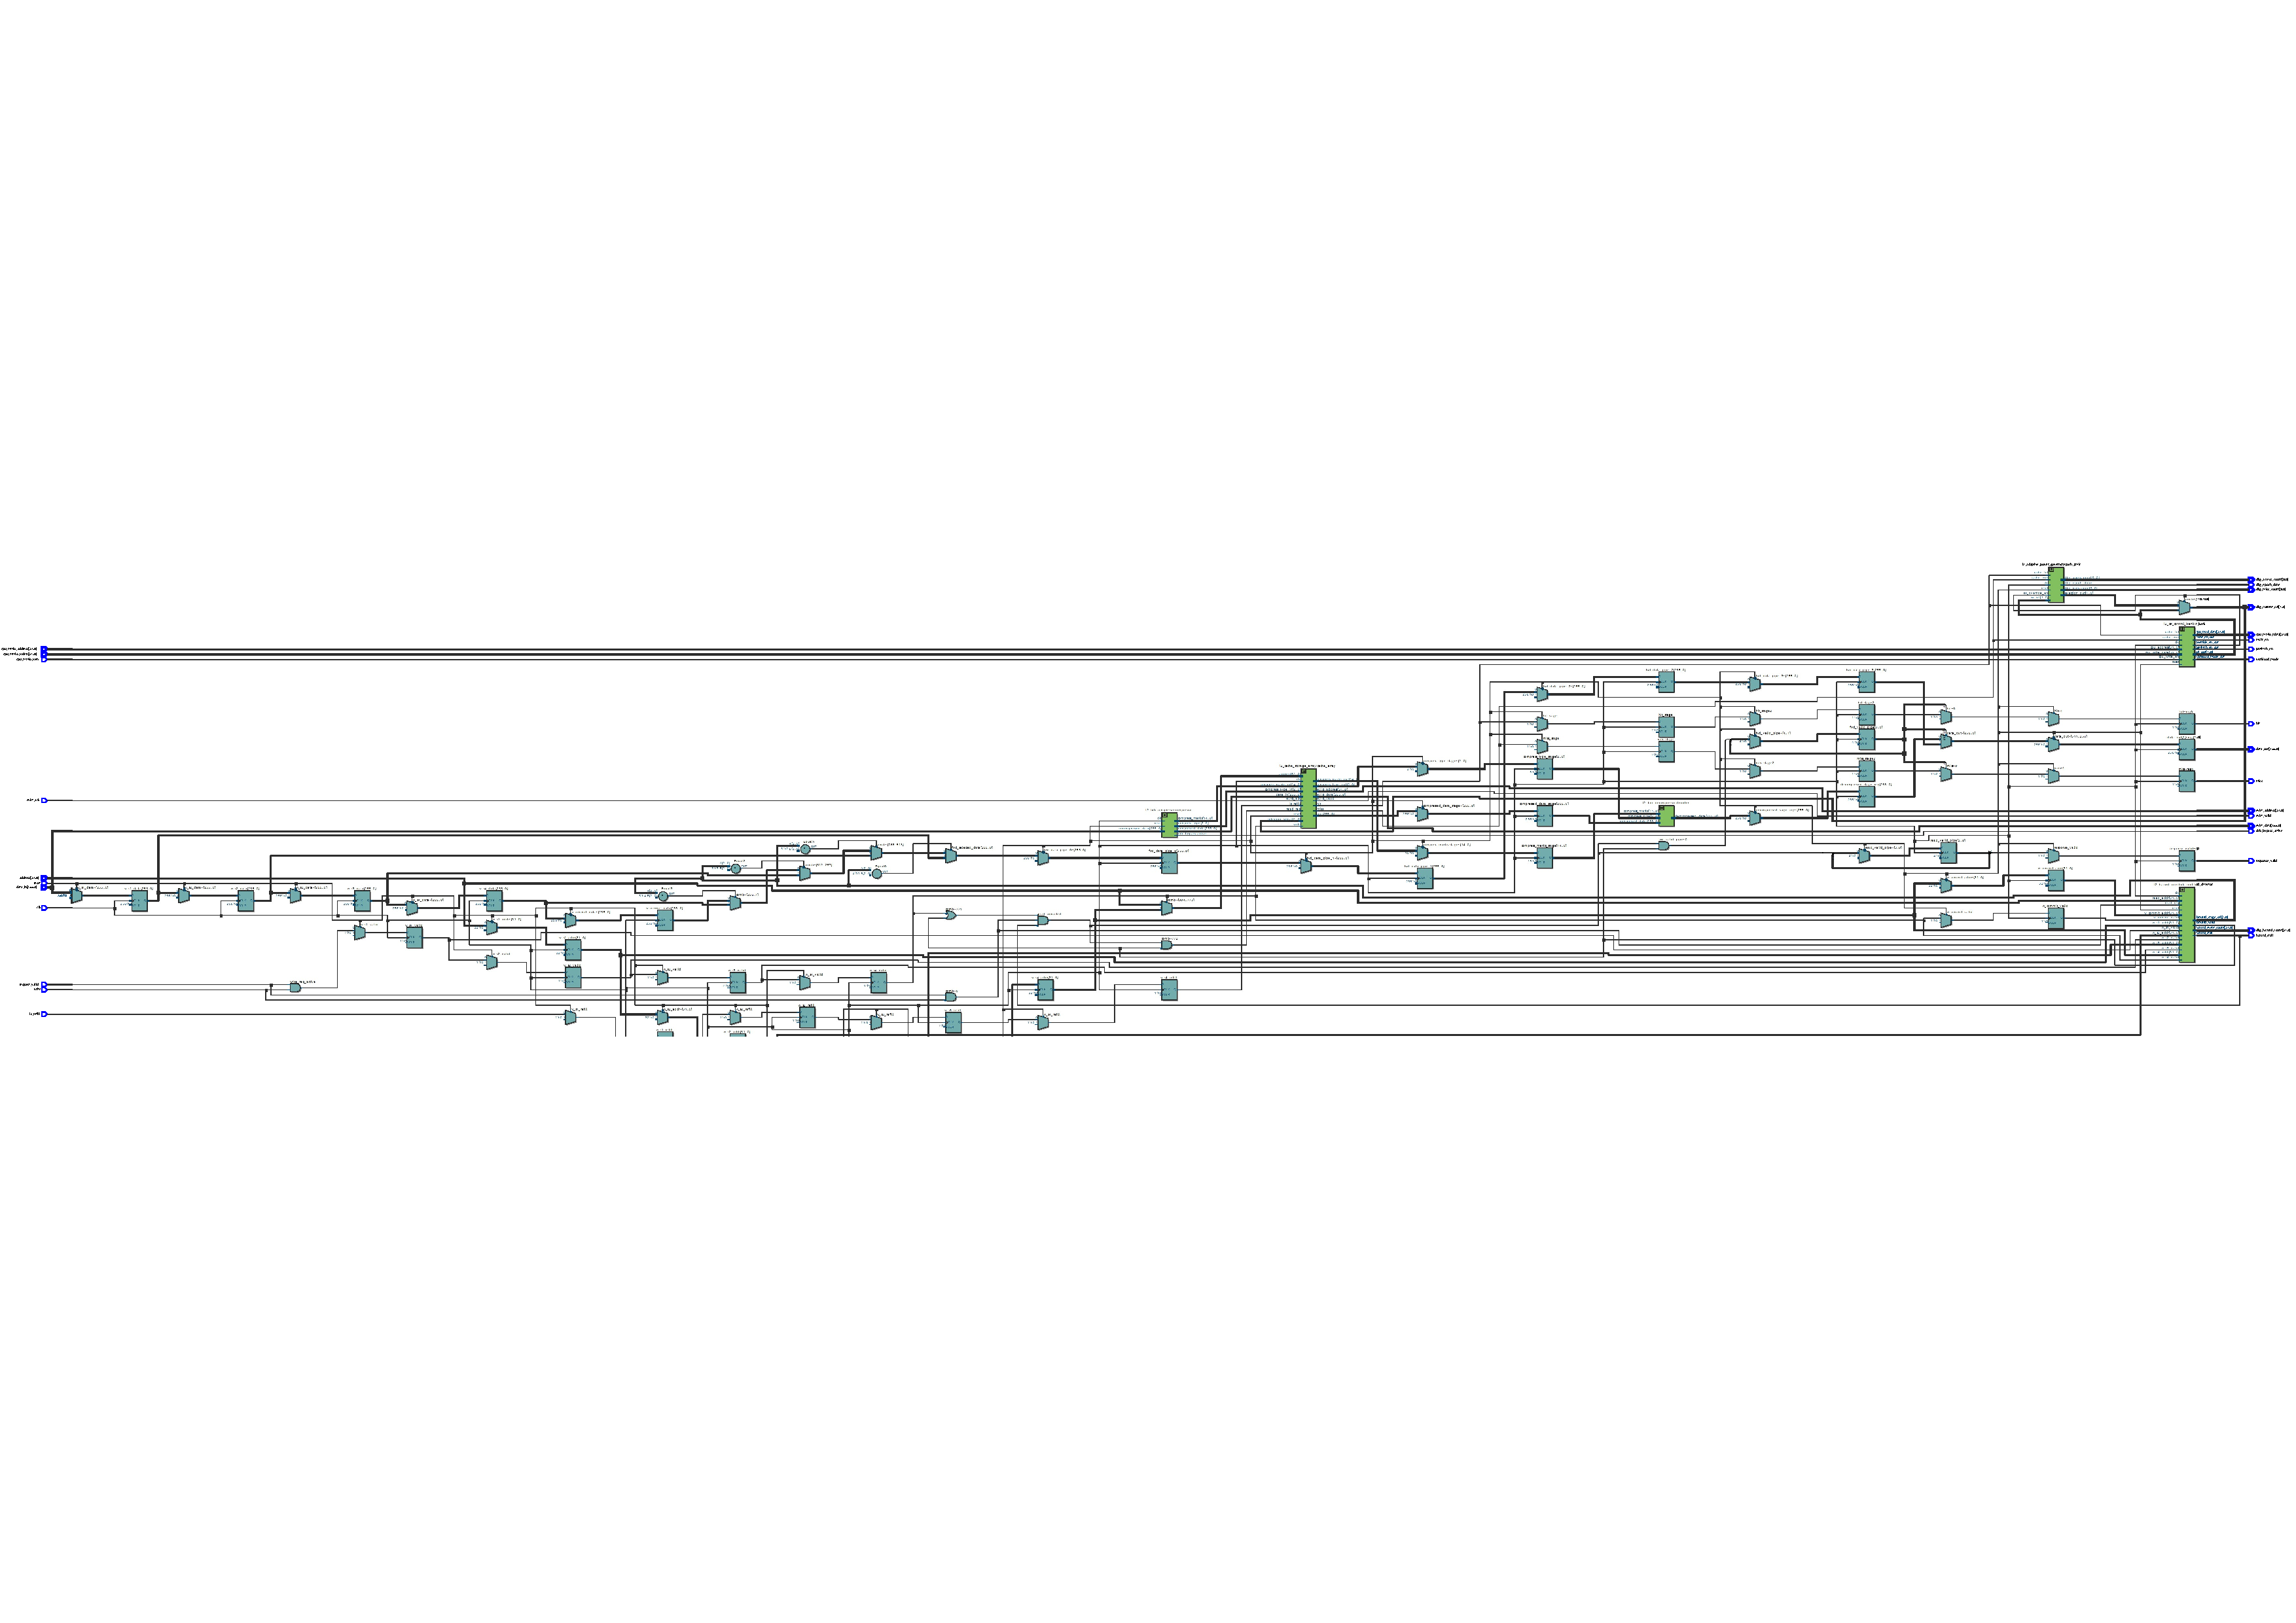
\includegraphics[width=1350mm, height=288mm, keepaspectratio]{assets/rtl_cropped.pdf}\par
        \vspace{2.0mm}
      \end{minipage}%
    }
  };

  % Right-1: Clean Compact Academic References (Width: 300mm, at x = 1424mm)
  \node[anchor=north west, inner sep=0pt, text width=300mm] at ([xshift=1424mm, yshift=-1118mm]current page.north west) {
    \noindent\fcolorbox{borderGray}{white}{%
      \begin{minipage}[c][318mm][c]{288mm}
        \vspace{2.0mm}
        {\fontsize{24pt}{29pt}\selectfont\spaceskip=0.33em\relax\textbf{\textcolor{navyDark}{\uppercase{Selected Academic References}}}}\par\vspace{4.5mm}
        {\fontsize{16pt}{22.5pt}\selectfont\spaceskip=0.33em\relax
        \hangindent=11mm\hangafter=1%
        \textbf{\textcolor{burgundy}{[1]}} G. Pekhimenko, V. Seshadri, O. Mutlu, P. B. Gibbons, M. A. Kozuch, and T. C. Mowry, ``Base-Delta-Immediate Compression: Practical Data Compression for On-Chip Caches,'' in \textit{Proc. 21st Int. Conf. Parallel Archit. Compil. Tech. (PACT)}, pp. 377--388, 2012.\par\vspace{3.6mm}
        \hangindent=11mm\hangafter=1%
        \textbf{\textcolor{burgundy}{[2]}} G. Pekhimenko, T. C. Mowry, and O. Mutlu, ``Line Distillation: Capacity-Versus-Bandwidth Tradeoff in Compressed Caches,'' \textit{IEEE Micro}, vol. 33, no. 3, pp. 26--35, 2013.\par\vspace{3.6mm}
        \hangindent=11mm\hangafter=1%
        \textbf{\textcolor{burgundy}{[3]}} A. R. Alameldeen and D. A. Wood, ``Adaptive Cache Compression for High-Performance Processors,'' in \textit{Proc. 31st Annual Int. Symp. Comput. Archit. (ISCA)}, pp. 212--223, 2004.\par\vspace{3.6mm}
        \hangindent=11mm\hangafter=1%
        \textbf{\textcolor{burgundy}{[4]}} S. Mittal, ``A Survey of Architectural Techniques for Improving Cache Power Efficiency,'' \textit{IEEE Trans. Very Large Scale Integr. (VLSI) Syst.}, vol. 22, no. 8, pp. 1827--1843, 2014.\par\vspace{3.6mm}
        \hangindent=11mm\hangafter=1%
        \textbf{\textcolor{burgundy}{[5]}} J. L. Hennessy and D. A. Patterson, \textit{Computer Architecture: A Quantitative Approach}, 6th ed., Cambridge, MA: Morgan Kaufmann / Elsevier, 2017.\par\vspace{3.6mm}
        \hangindent=11mm\hangafter=1%
        \textbf{\textcolor{burgundy}{[6]}} I. Kuon and J. Rose, ``Measuring the Gap Between FPGAs and ASICs,'' \textit{IEEE Trans. Comput.-Aided Design Integr. Circuits Syst.}, vol. 26, no. 2, pp. 203--215, 2007.\par\vspace{3.6mm}
        \hangindent=11mm\hangafter=1%
        \textbf{\textcolor{burgundy}{[7]}} N. H. E. Weste and D. M. Harris, \textit{CMOS VLSI Design: A Circuits and Systems Perspective}, 4th ed., Boston, MA: Addison-Wesley / Pearson, 2010.\par\vspace{3.6mm}
        \hangindent=11mm\hangafter=1%
        \textbf{\textcolor{burgundy}{[8]}} Intel Corporation, \textit{Cyclone IV Device Handbook: Volume 1 --- Embedded Memory Blocks (M9K) and Clock Networks}, San Jose, CA: Intel PSG, 2020.\par
        }
        \vspace{2.0mm}
      \end{minipage}%
    }
  };

  % Right-2: Clean Proportional QR Code Card (Width: 222mm, at x = 1740mm)
  \node[anchor=north west, inner sep=0pt, text width=222mm] at ([xshift=1740mm, yshift=-1118mm]current page.north west) {
    \noindent\fcolorbox{borderGray}{white}{%
      \begin{minipage}[c][318mm][c]{210mm}
        \vspace{3.0mm}
        \centering
        {\fontsize{22pt}{26pt}\selectfont\spaceskip=0.33em\relax\textbf{\textcolor{burgundy}{\uppercase{Hardware Repository}}}}\par\vspace{2.5mm}
        {\fontsize{16pt}{20pt}\selectfont\spaceskip=0.33em\relax\textbf{\textcolor{navyDark}{IEEE 1364 Verilog RTL \& Testbenches}}}\par\vspace{4.0mm}
        
\includegraphics[width=182mm, height=182mm, keepaspectratio]{assets/qr_code.png}\par\vspace{4.0mm}
        {\fontsize{15.5pt}{19.5pt}\selectfont\texttt{\textbf{\textcolor{navyDark}{github.com/mohammed-gweaa/\allowbreak compressed-cache-fpga}}}}\par\vspace{2.5mm}
        {\fontsize{14pt}{18pt}\selectfont\spaceskip=0.33em\relax\textcolor{mutedGray}{\textbf{Scan for Full ModelSim Waves \& Synthesis Scripts}}}\par
        \vspace{2.0mm}
      \end{minipage}%
    }
  };

  % =========================================================================
  % 5. INSTITUTIONAL FOOTER BAR (Height: 38.5mm, at bottom)
  % =========================================================================
  % Gold top border (5.5mm)
  \fill[gold] (current page.south west) ++(0, 38.5mm) rectangle ++(2000mm, 5.5mm);
  
  % Burgundy background (38.5mm)
  \fill[burgundy] (current page.south west) rectangle ++(2000mm, 38.5mm);

  % Footer single-line container with perfect spacing across full width
  \node[anchor=south west, inner sep=0pt, text width=2000mm] at (current page.south west) {
    \begin{minipage}[c][38.5mm][c]{2000mm}
      \hspace{38mm}%
      {\fontsize{24pt}{29pt}\selectfont\spaceskip=0.33em\relax\textbf{\textcolor{white}{Department of Computer Engineering $\cdot$ Faculty of Engineering $\cdot$ University of Tripoli $\cdot$ Academic Year 2025--2026}}}%
      \hfill%
      {\fontsize{24pt}{29pt}\selectfont\spaceskip=0.33em\relax\textbf{\texttt{\textcolor{footerHighlight}{TARGET SILICON: INTEL CYCLONE IV GX EP4CGX150DF31C7 $\cdot$ TIMING CLOSED @ 50 MHz (+3.218 ns SLACK) $\cdot$ 100\% ASSERTIONS PASSED}}}}%
      \hfill%
      {\fontsize{24pt}{29pt}\selectfont\spaceskip=0.33em\relax\textbf{\textcolor{white}{Intel Quartus Prime 22.1std $\cdot$ TimeQuest STA $\cdot$ Mentor ModelSim 2020.1}}}%
      \hspace{38mm}
    \end{minipage}
  };

\end{tikzpicture}
\end{document}
